%!TeX root=../tcc.tex

%% ------------------------------------------------------------------------- %%
\chapter{Ordenação cinética}
Considere o seguinte problema cinético. São dados $n$ pares de
valores. Cada par $(x_0, v)$ representa um valor que está mudando
linearmente com o tempo. Num instante arbitrário $t \geq 0$, o valor
correspondente ao par $(x_0, v)$ é $x_0 + tv$. O objetivo é
responder consultas do tipo: para um certo $i$, com $1 \leq i \leq
n$, quem é o $i$-ésimo maior valor da coleção no instante corrente.

Por exemplo, se tivermos quatro elementos na coleção, digamos
$\left(6, -\frac{1}{2}\right)$, $(5, 0)$, $\left(3,
\frac{1}{4}\right)$ e $\left(0, \frac{4}{3}\right)$, podemos
representar essa coleção como na figura \ref{fig:ordenacao:exemplo}.

\begin{figure}[H]
    \centering
    \begin{figure}[H]
    \centering
    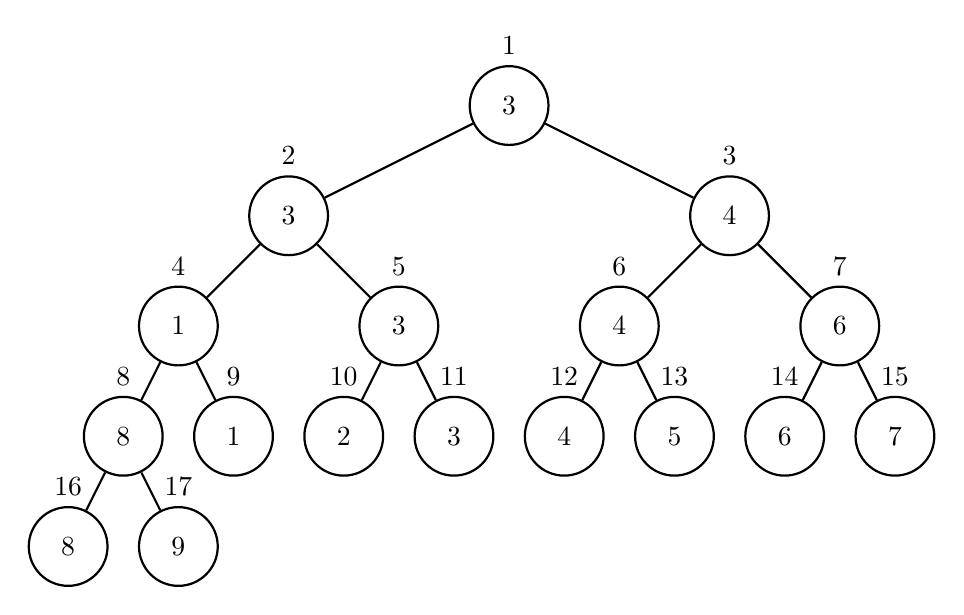
\begin{tikzpicture}[thick, scale=0.7]
        \node[label={1},circle,draw,minimum size=1cm]
        (1) at (0,0) {$3$};
        \node[label={2},circle,draw,minimum size=1cm]
        (2) at (-4,-2) {$3$};
        \node[label={3},circle,draw,minimum size=1cm]
        (3) at (4,-2) {$4$};
        \node[label={4},circle,draw,minimum size=1cm]
        (4) at (-6,-4) {$1$};
        \node[label={5},circle,draw,minimum size=1cm]
        (5) at (-2,-4) {$3$};
        \node[label={6},circle,draw,minimum size=1cm]
        (6) at (2,-4) {$4$};
        \node[label={7},circle,draw,minimum size=1cm]
        (7) at (6,-4) {$6$};
        \node[label={8},circle,draw,minimum size=1cm]
        (8) at (-7,-6) {$8$};
        \node[label={9},circle,draw,minimum size=1cm]
        (9) at (-5,-6) {$1$};
        \node[label={10},circle,draw,minimum size=1cm]
        (10) at (-3,-6) {$2$};
        \node[label={11},circle,draw,minimum size=1cm]
        (11) at (-1,-6) {$3$};
        \node[label={12},circle,draw,minimum size=1cm]
        (12) at (1,-6) {$4$};
        \node[label={13},circle,draw,minimum size=1cm]
        (13) at (3,-6) {$5$};
        \node[label={14},circle,draw,minimum size=1cm]
        (14) at (5,-6) {$6$};
        \node[label={15},circle,draw,minimum size=1cm]
        (15) at (7,-6) {$7$};
        \node[label={16},circle,draw,minimum size=1cm]
        (16) at (-8,-8) {$8$};
        \node[label={17},circle,draw,minimum size=1cm]
        (17) at (-6,-8) {$9$};

        \draw[thick] (1) -- (2);
        \draw[thick] (2) -- (4);
        \draw[thick] (4) -- (8);
        \draw[thick] (4) -- (9);
        \draw[thick] (8) -- (16);
        \draw[thick] (8) -- (17);
        \draw[thick] (2) -- (5);
        \draw[thick] (5) -- (10);
        \draw[thick] (5) -- (11);
        \draw[thick] (1) -- (3);
        \draw[thick] (3) -- (6);
        \draw[thick] (3) -- (7);
        \draw[thick] (6) -- (12);
        \draw[thick] (6) -- (13);
        \draw[thick] (7) -- (14);
        \draw[thick] (7) -- (15);
    \end{tikzpicture}
    \caption[Representação da estrutura torneio]{Torneio com $9$
        elementos em que $3$ é o elemento com valor máximo.}
    \label{fig:torneio:exemplo}
\end{figure}
    \caption[Exemplo ordenação cinética]{O segundo maior valor no
            instante $t = 0$ é do elemento $2$, e no instante $t =
            3$ é do elemento $1$. O menor valor da coleção no
            instante $t = 3$ é do elemento $3$, e no instante $t =
            5$ é do elemento $1$.}
    \label{fig:ordenacao:exemplo}
\end{figure}

Queremos dar suporte às seguintes operações:
\begin{itemize}
    \item \textsc{advance}$(t)$ $\rightarrow$ avança o tempo
    corrente para $t$;
    \item \textsc{change}$(j, v)$ $\rightarrow$ altera a
    velocidade do elemento $j$ para $v$;
    \item \textsc{query\_kth}$(i)$ $\rightarrow$ devolve o
    elemento cujo valor é o $i$-ésimo maior no instante atual.
\end{itemize}